%%%%%%%%%%%%%%%%%%%%%%%%%%%%%%%%%%%%%%%%%%%%%%%%%%%%%%%%%%%%%%%%%%%%%%%%%%%%%%%%%%%%%%%%%%%%%%%%%%%%%%%%%%%%%%%%%%%%%%%%%%%%%%%%%%%%%%%%%%%%%%%%%%%%%%%%%%%
% This is just an example/guide for you to refer to when submitting manuscripts to Frontiers, it is not mandatory to use Frontiers .cls files nor frontiers.tex  %
% This will only generate the Manuscript, the final article will be typeset by Frontiers after acceptance.
%                                              %
%                                                                                                                                                         %
% When submitting your files, remember to upload this *tex file, the pdf generated with it, the *bib file (if bibliography is not within the *tex) and all the figures.
%%%%%%%%%%%%%%%%%%%%%%%%%%%%%%%%%%%%%%%%%%%%%%%%%%%%%%%%%%%%%%%%%%%%%%%%%%%%%%%%%%%%%%%%%%%%%%%%%%%%%%%%%%%%%%%%%%%%%%%%%%%%%%%%%%%%%%%%%%%%%%%%%%%%%%%%%%%

%%% Version 3.4 Generated 2018/06/15 %%%
%%% You will need to have the following packages installed: datetime, fmtcount, etoolbox, fcprefix, which are normally inlcuded in WinEdt. %%%
%%% In http://www.ctan.org/ you can find the packages and how to install them, if necessary. %%%
%%%  NB logo1.jpg is required in the path in order to correctly compile front page header %%%

\documentclass[utf8]{FrontiersinHarvard} % for articles in journals using the Harvard Referencing Style (Author-Date), for Frontiers Reference Styles by Journal: https://zendesk.frontiersin.org/hc/en-us/articles/360017860337-Frontiers-Reference-Styles-by-Journal
%\documentclass[utf8]{FrontiersinVancouver} % for articles in journals using the Vancouver Reference Style (Numbered), for Frontiers Reference Styles by Journal: https://zendesk.frontiersin.org/hc/en-us/articles/360017860337-Frontiers-Reference-Styles-by-Journal
%\documentclass[utf8]{frontiersinFPHY_FAMS} % Vancouver Reference Style (Numbered) for articles in the journals "Frontiers in Physics" and "Frontiers in Applied Mathematics and Statistics"

%\setcitestyle{square} % for articles in the journals "Frontiers in Physics" and "Frontiers in Applied Mathematics and Statistics"
\usepackage{url,hyperref,lineno,microtype,subcaption}
\usepackage[onehalfspacing]{setspace}
\captionsetup{compatibility=false}

\linenumbers
% Leave a blank line between paragraphs instead of using \\


%\def\keyFont{\fontsize{8}{11}\helveticabold }
%\def\firstAuthorLast{Sample {et~al.}} %use et al only if is more than 1 author
%\def\Authors{Sunil Kumar Vengalil\,$^{1,*}$, Bharath K\,$^{2}$ and Neelam Sinha\,$^{1,2}$}
%% Affiliations should be keyed to the author's name with superscript numbers and be listed as follows: Laboratory, Institute, Department, Organization, City, State abbreviation (USA, Canada, Australia), and Country (without detailed address information such as city zip codes or street names).
%% If one of the authors has a change of address, list the new address below the correspondence details using a superscript symbol and use the same symbol to indicate the author in the author list.
%\def\Address{$^{1}$ International Institute of Information Technology Bangalore, Bangalore, India \\
%% $^{2}$Laboratory X, Institute X, Department X, Organization X, City X , State XX (only USA, Canada and Australia), Country X  }
%% The Corresponding Author should be marked with an asterisk
%% Provide the exact contact address (this time including street name and city zip code) and email of the corresponding author
%\def\corrAuthor{Sunil Kumar Vengalil}
%
%\def\corrEmail{sunilkumar.vengalil@iiitb.ac.in}

\def\keyFont{\fontsize{8}{11}\helveticabold }
\def\firstAuthorLast{Sunil Vengalil {et~al.}} %use et al only if is more than 1 author
\def\Authors{Sunil Kumar Vengalil\,$^{*}$, Bharath K, and Neelam Sinha}
% Affiliations should be keyed to the author's name with superscript numbers and be listed as follows: Laboratory, Institute, Department, Organization, City, State abbreviation (USA, Canada, Australia), and Country (without detailed address information such as city zip codes or street names).
% If one of the authors has a change of address, list the new address below the correspondence details using a superscript symbol and use the same symbol to indicate the author in the author list.
\def\Address{International Institute of Information Technology Bangalore, Bangalore, India }
% The Corresponding Author should be marked with an asterisk
% Provide the exact contact address (this time including street name and city zip code) and email of the corresponding author
\def\corrAuthor{Sunil Kumar Vengalil}

\def\corrEmail{sunilkumar.vengalil@iiitb.ac.in}



\begin{document}
\onecolumn
\firstpage{1}

\title[Simultaneous Segmentation of Multiple Structures in Fundal Images using DNN]{Simultaneous Segmentation of Multiple Structures in Fundal Images using Multi-tasking Deep Neural Networks}

\author[\firstAuthorLast ]{\Authors} %This field will be automatically populated
\address{} %This field will be automatically populated
\correspondance{} %This field will be automatically populated

\extraAuth{}% If there are more than 1 corresponding author, comment this line and uncomment the next one.
%\extraAuth{corresponding Author2 \\ Laboratory X2, Institute X2, Department X2, Organization X2, Street X2, City X2 , State XX2 (only USA, Canada and Australia), Zip Code2, X2 Country X2, email2@uni2.edu}

\maketitle


\begin{abstract}

%%% Leave the Abstract empty if your article does not require one, please see the Summary Table for full details.
\section{}
Fundal imaging is the most commonly used non-invasive technique for early detection of many retinal diseases like Diabetic Retinopathy(DR). An initial step in automatic processing of fundal images for detecting diseases is to identify the normal landmarks: Optic Disc, Blood Vessels and Macula.   In addition to these, various abnormalities like exudates that help in pathological analysis are also visible in fundal images. In this work, we propose a multi-tasking deep learning architecture for segmenting Optic Disc, Blood Vessels, Macula and exudates simultaneously. The objective is to improve the prediction results on Blood Vessels and exudates, which are relatively more challenging, while utilizing segmentation of Optic Disc and Macula as auxiliary tasks. Our experimental results on publicly available datasets show that simultaneous segmentation of all these structures results in significant improvement in the performance. Among the segmented structures maximal improvement of 15\% is obtained on exudates when trained using multi-tasking loss function.  The proposed approach makes predictions for the whole image in a single forward pass.  We use  modified U-Net architecture with only convolutional and de-convolutional layers with comparatively less number of parameters leading to faster (by a factor of 12) prediction time, compared to the current AUC-wise best performing exudate segmentation deep learning model, ERUnet. The proposed approach has been evaluated on publicly available datasets DRIVE, HRF, CHASE\_DB and IDRiD datasets. Comparison of results with the state-of-the-art have also been presented.
\tiny
\keyFont{ \section{Keywords:} Fundal Image Segmentation, Deep Learning, Multi-task learning, Exudates Segmentation, Blood Vessels, Macula, Optic Disc }
\end{abstract}

\section{Introduction}

Fundal imaging, capturing images of retina using specialized cameras, is the most widely used non-invasive technique for screening of retinal diseases. These images are used to identify common eye diseases like Diabetic Retinopathy (DR) \cite{hu2015curbing} and Glaucoma which are the most common cause for blindness and could be indicators of many other cardiovascular diseases. Blood Vessels (BV), Optic Disc (OD) and Macula are the normal landmarks visible in a healthy fundal image. Certain features of BV like tortuosity are widely used for early detection of various cardio-vascular diseases \cite{krestanova2020recent}. However, manual identification and demarcation of fine structures like BV require domain expertise, besides being prone to manual errors. Features extracted for OD like, Cup-to-Disc ratio can be used for detection of Glaucoma. Hence automatic detection of major landmarks in fundal image has become an active research area \cite{kou2020enhanced,guo2020bin,nur2018exudate,jiang2018retinal, joshua2020blood, dash2020retinal}.

Figure \ref{fig:sample_funal_image} shows a fundal image with normal landmarks like BV, OD and Macula marked. The OD is the point of exit of the optic nerves that carry information from the eye to the brain. It is also the point where all the BV enter the eye. Since there are no photo sensors (rods and cones) present in the OD, it corresponds to a blind spot in the retina. Macula is a small region with a lot of cone cells packed together and hence this region is responsible for sharp vision \cite{maculaurl}. The center point of Macula is called Fovea. BV that carry blood to the eye are spread across the entire region of the retina and vary in thickness and density.

\begin{figure}
\centering
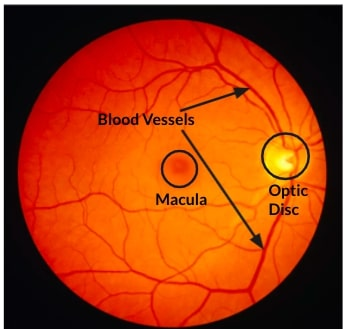
\includegraphics[width=0.5\linewidth]{images/fundal_fovea_bv_od.jpg}
\caption{Sample fundal image showing normal landmarks BV, OD and Macula}
\label{fig:sample_funal_image}
\end{figure}

Figures \ref{fig:exudates_with_gt}a and \ref{fig:exudates_with_gt}b show a sample  fundal image with exudates and its corresponding ground truth. Exudates are the fluid (pus) leaking out of Blood Vessels. It is indicative of advanced stage of Diabetic Retinopathy. Exudates appear as unstructured, scattered, bright patches in the fundal image.

\begin{figure}
\centering
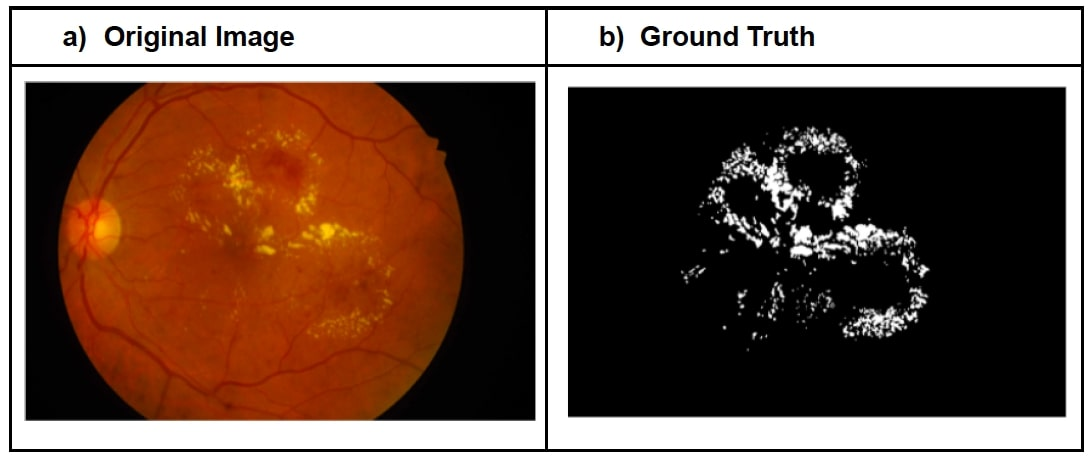
\includegraphics[width=0.8\linewidth]{images/exudates_with_gt.jpg}
\caption{Sample fundal image with exudates and corresponding ground truth image for exudates}
\label{fig:exudates_with_gt}
\end{figure}

Since the break-through success of deep learning in solving tasks in domains like computer vision for classification \cite{krizhevsky2012imagenet} \cite{simonyan2014very} the framework has been successfully extended to more complex tasks such as semantic segmentation \cite{chen2017deeplab,Yu_2018_ECCV,wang2018under} . Many deep learning architectures have been utilized for segmenting challenging structures, such as BV \cite {vengalil2016customizing} \cite{zhuang2018laddernet} \cite{jiang2018retinal} \cite{park2020m} and exudates \cite{kou2020enhanced,guo2020bin,nur2018exudate} in fundal images. One of the issues in using deep learning architecture for medical images is limited availability  of annotated training data. Many approaches, like taking multiple training patches from  a single image \cite{vengalil2016customizing} and transfer learning \cite{vengalil2016customizing}, have been successfully explored.

In this work, we propose a multi-tasking deep learning architecture for simultaneous segmentation of BV, OD, Macula and exudates. Our results show that a single network that predicts multiple structures  performs better compared to detecting  each structure independently using different networks, as the single network can make use of the correlation between the multiple tasks. This correlation is evident from Figure \ref{fig:sample_funal_image}, where it is clear that BV is thicker and denser near and inside the OD. So the task of the OD segmentation can help the segmentation task for BV and vice versa.  Similarly, the relative position of OD and Macula can help to improve the segmentation performance of each of these structures. We perform experiments and report results on four popular datasets DRIVE , HRF \cite{budai2013robust}, CHASE\_DB and IDRiD \cite{h25w98-18}.

We use publicly available and well evaluated datasets, namely DRIVE, HRF and CHASE\_DB, for our studies on BV segmentation. Since the number of images in these datasets are relatively less (40, 45 and 28 respectively for the above mentioned datasets), we use data augmentation techniques such as horizontal flip, vertical flip, rotations, elastic transformation, grid distortion and optic distortion to increase the number of training images by a factor 4-6. The major contribution of this work is to propose a multi-tasking model for simultaneous segmentation of BV, OD, Macula and exudates. The proposed multi-tasking model resulted in an improvement of F1 score by 15\% for exudates besides being faster (by a factor of 12).

\section{Related Work}
\subsection{Blood Vessel Segmentation}
Existing  techniques for fundal image segmentation mainly fall under two categories 1) using traditional image processing techniques and 2) using deep learning techniques. Examples of image processing based techniques include filter based: \cite{zhang2010retinal}, \cite{yavuz2011retinal} and \cite{aslan2018segmentation} and morphological operations based \cite{hassan2015retinal} and \cite{singh2014new}. Image processing based techniques have the advantage that domain knowledge can be easily incorporated through hand crafted features, however they are not easily generalizable across diverse datasets. Further, these algorithms are based on many customized parameters that may vary from dataset to dataset. Generalization becomes challenging since there could be hardware differences, change in acquisition conditions, different pathologies etc.

Several deep learning architectures, that were successful in segmentation tasks (\cite{chen2017deeplab}) in natural images, were tried for segmenting Blood Vessels in retinal images and the results were significantly better than using conventional image processing techniques. \cite{vengalil2016customizing} used a popular segmentation model deeplab (\cite{chen2017deeplab}) which was pre-trained on natural images  for semantic segmentation,   to segment Blood Vessels at pixel level. \cite {jiang2018retinal} proposes a  pre-trained fully convolutional network for segmenting BV and reports accuracy of cross-dataset test on four different datasets. In M-GAN, proposed by \cite{park2020m}, a multi-kernel pooling block added between stacked convolutional layers supports scale-invariance which is a highly desirable feature for BV segmentation.

One of the main challenges in using deep neural networks for segmentation tasks is that the reduction in resolution of featuremap as one goes deeper will result in loss of finer details like edges, which are crucial for segmentation tasks. In order to circumvent this, the U-Net( \cite{ronneberger2015u}) model was introduced specifically for medical image segmentation which has multiple skip connections. In their recent work, Joshua et.al. \cite{joshua2020blood} used a modified version of U-NET for segmenting BV in retinal images and reported state-of-the-art accuracies. Laddernet, introduced by Zhuang et.al. in 2018 \cite{zhuang2018laddernet},  is a sequence of multiple U-Nets cascaded together.

\subsection{Exudates Segmentation}
Like BV segmentation, reported studies on exudates segmentation  were also performed both using traditional image processing techniques \cite{}  and deep learning techniques . Existing works on exudates segmentation using deep learning approaches include \cite{perdomo2017convolutional,tan2017automated, feng2017deep, zheng2018detection}. The work reported in \cite{perdomo2017convolutional,kou2020enhanced} used a convolutional neural network,  LeNet \cite{lecun1989handwritten}, to classify patches extracted from fundal images into classes of ``with exudates" or ``without exudates". They extract patches of size $48\times48$ and hence the network does not provide a pixel-wise segmentation.  The work reported in \cite{kou2020enhanced} proposed a deep learning approach, called Enhanced Residual U-Net (ERU-Net). Their proposed model had three U-paths each with three upsampling paths and one downsampling path. This structure enhances the feature fusion capability of the networks capturing more details of fundal image. The proposed model also made use of residual blocks.


\section{Proposed Method}
\subsection{CNN architecture}

\begin{figure}
\centering
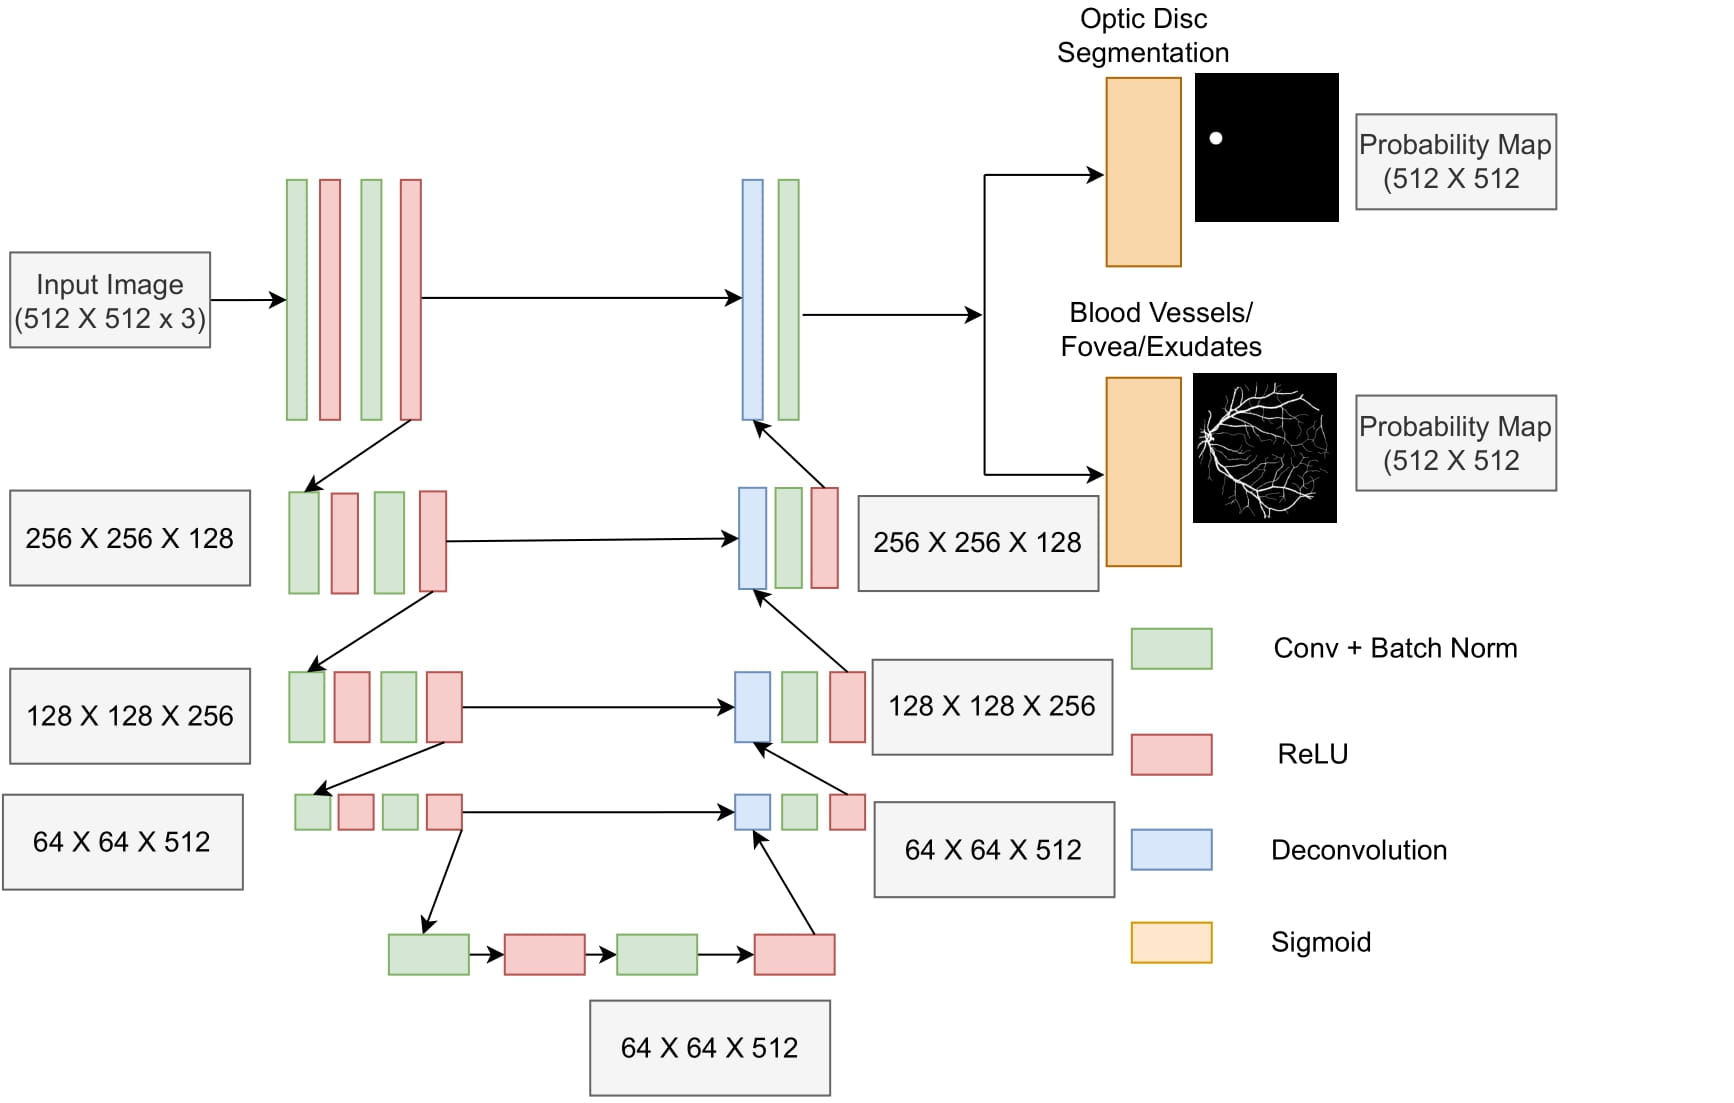
\includegraphics[width=0.9\linewidth]{images/UnetArch.jpg}
\caption{Architecture of the proposed multi-tasking U-Net model}
\label{unet_combined}
\end{figure}

A modified version of the UNET architecture proposed by \cite{ronneberger2015u}, shown in Fig \ref{unet_combined}, is used for segmenting various structures. The modifications are:
\begin{enumerate}
\item Our proposed network retains the original dimensions of the input image, whereas the original U-Net mentioned in \cite{ronneberger2015u} reduced the original  input size from $572 \times 572$ to $388 \times 388$.

\item We use de-convolutional layers with a stride of 2 for up-sampling as opposed to  upsampling layers used in original U-Net architecture. Our method has the advantage that the network also learns the interpolation weights using a deconvolutional layer.
\item We add batch normalization after each convolutional layer in order to stabilize the training process as well as for faster training.
\end{enumerate}

The encoder and decoder consists of 4 stages each. Each stage of the encoder comprises two convolution layers, each followed by batch normalization and ReLU activation function. A max-pooling layer with a stride of 2 was added at the end of each stage of the encoder which down samples the image by a factor of two.
Each decoder layer up-samples the image by a factor of 2 using  a deconvolution layer followed by a convolution layer. The sigmoid function is used in the final output channel with two filters instead of the softmax activation function because the BV and OD features are not  mutually exclusive. These features share common connections in the fundal image, and hence, their simultaneous segmentation also yields the best results.

For multi-tasking experiments, the auxiliary task chosen was Optic Disc segmentation. We also evaluate models with different dimensions of latent representation and different number of channels  in the bottleneck layer and report the results for all combinations. For latent representation dimension, we experimented with different values $16\times16$, $32\times32$, $64\times64$ and $128\times128$. For the number of channels, experiments are carried out with 384, 512, 768, 1024 and 1280.

\subsection{Dataset}
We use the DRIVE, HRF \cite{budai2013robust}, CHASE\_DB and IDRiD \cite{h25w98-18}, datasets. The DRIVE dataset contains 20 training images and 20 testing images of resolution $565 \times 584$ pixels. The dataset also provides ground truth images for BV segmentation annotated by a human expert. As the DRIVE and CHASE\_DB dataset does not have Optic Disc annotations, we annotated the Optic Disc in each image ourselves. HRF dataset has 15 high resolution fundal images along with ground truth annotation for BV segmentation.

IDRiD, \cite{h25w98-18}, localization dataset which contains 413 training images and 103 test images along with Fovea ground truth, was used for Macula localization. For exudates segmentation, we used the IDRiD segmentation dataset which contains a total of 81 images. OD ground truth is available as part of the dataset but BV ground truths are not available. For training exudates in multi-tasking mode, we first predicted BV segmentation on these images using model trained on images taken from HRF, DRIVE and CHASE\_DB datasets. These  predictions were used as BV ground truth for multi-tasking training.

Data-augmentation: horizontal and vertical flipping, grid and elastic distortion provided by the library Albumentations, \cite{buslaev2020albumentations}, was used  to increase the number of training samples by a factor of 4.

No pre-processing, other than resizing the images to $512\times512$, was performed on the original images.

\subsection{Experiments performed}
We use full images, as opposed to image patches, for training the network  as a full image will have more context and hence can be more effective for predicting structures like Optic Disc and Macula. We perform multiple experiments, for individual and simultaneous prediction of Blood Vessels, Optic Disc, Macula and exudates.

To start with, we perform BV segmentations on the individual datasets with the proposed U-Net architecture to achieve the best possible results. To further improve the results obtained on the Blood Vessels, we utilize simultaneous segmentation of Blood Vessels and Optic Disc. Apart from these experiments, we also modify the U-Net architecture to find the best suitable parameters for both Blood Vessels and Optic Disc.

Another experiment we carried out is to train a model for BV segmentation using training set containing images from HRF, DRIVE and CHASE datasets and we evaluate the performance of this trained model on  1) on a held out validation dataset which comprises images from HRF, DRIVE and CHASE\_DB  2) test dataset containing images from IDRiD dataset. On the IDRiD dataset, we evaluate the model qualitatively as no ground truth was available for this dataset. Further in order to measure the generalizability of the trained model we also report across the dataset results for all tasks.

The obtained BV results on the IDRiD dataset is further utilized to improve the Optic Disc, Macula and exudates segmentation results.

\subsection{Loss function and training}\label{sec:loss_and_training}
A sigmoid activation function is used at the output layer. The model is trained with dice loss and  with a combination of dice loss and binary cross entropy loss. In most of the experiments, we noticed that the combination of two losses gave a better F1-score.

For predicting the structures separately, four separate networks with the same architecture are trained independently one for each of the structures: Blood Vessel, Optic Disc, Macula and exudates.

In the multi-tasking model, we train three separate networks each with two output channels, for predicting the following three combinations:
\begin{enumerate}
\item BV and OD
\item Macula and OD
\item Exudates and OD
\item BV and Macula
\item BV and exudates
\item Exudates, BV and OD
\item Macula, BV and OD
\end{enumerate}

The network is trained for 60 epochs in all the cases.

\section{Results and Discussion}\label{sec:results}

\begin{table}[!h]
\caption{Comparison of results with and without multi-tasking. For all the tasks except OD, multi-tasking was done with OD as an auxiliary task. For OD, multi-tasking was done in combination with Blood Vessels.}
\begin{center}
\begin{tabular}{|c|c|c|c|c|c|}
\hline
&&\multicolumn{2}{|c|}{\textbf{Individual}}& \multicolumn{2}{|c|}{\textbf{Multi-tasking}} \\
\cline{3-6}
&\textbf{\textit{Dataset}}& \textbf{\textit{Dice(\%)}}& \textbf{\textit{IoU(\%)}}& \textbf{\textit{Dice(\%)}}& \textbf{\textit{IoU(\%)}}  \\
\hline
Blood Vessel & DRIVE & 77.00 & 62.78 & 80.31 & 67.35  \\
\cline{2-6}
& HRF & 78.11 & 64.29 & 81.66 & 69.04 \\
\cline{2-6}
& CHASE\_DB & 74.34 & 59.21 & 80.45 & 67.32 \\
\hline
Optic Disc & DRIVE & 76.24 & 66.15 & 78.63 & 69.85  \\
\cline{2-6}
&IDRiD & 85.73 & 64.65 & 94.51 & 89.98 \\
\hline
Macula & IDRiD & 68.13 & 60.16 & 70.52 &  61.77 \\
\hline
exudates & IDRiD & 50.34 & 34.56 & 61.37 & 46.33  \\
\hline
\end{tabular}
\label{tab:results}
\end{center}
\end{table}

For comparison of multi-tasking segmentation with segmentation of individual structures, experiments on individual prediction were performed. In this case, the network had one output channel corresponding to the segmentation map. The network outputs a binary image, of the same resolution as the input,  which indicates pixel by pixel segmentation. For multi-tasking models, additional channels for predicting additional structures  in combination with another structure are added at the output layer.

Table \ref{tab:results} compares segmentation performance of various structures when the model is trained with and without multi-tasking. The table provides a comparison of  results when  the model is trained in multi-tasking mode with two different tasks  Vs the results with an individual task. In all these cases, OD is added as an auxiliary task along with other main tasks like BV, Macula and exudates. The row for OD shows comparison of segmentation performance of OD when trained with OD alone Vs results of multi-tasking loss with BV.  As evident from the table, Dice score for exudates segmentation resulted in an improvement  of 10\% when the model was trained in combination with Optic Disc. A similar trend is observed in BV and OD segmentation with an improved Dice score of about 4\% (for HRF) and 6\% (for CHASE\_DB). For Macula, the segmentation results decreased by 2\% upon addition of Optic Disc as an additional task during training. This happens because the Macula and Optic Disc are mutually exclusive as they appear at different locations in the image. In all our simultaneous segmentation experiments we use sigmoid as output activation function which is used for multi-label prediction which is not true in this case. However, when trained with Blood Vessels, Macula and OD together we observed a 3\% increase in the score for Macula.

\begin{table}
\caption{Results of various multi-tasking experiments run on segmentation of exudates. We got the best results when the model is trained with multi-tasking loss for a combination of exudates, OD and BV.}
\begin{center}
\begin{tabular}{ |l|c|c|  }
\hline
\textbf{Experiments Run} & \textbf{Dice(\%)} & \textbf{AUC}\\
\hline
Exudates Alone & 50.34 & 0.8402 \\
\hline
Exudates and OD & 53.32 & 0.8078\\
\hline
Exudates and BV & 61.37 & 0.8365\\
\hline
\textbf{Exudates, OD and BV} & \textbf{65.00} & \textbf{0.9993} \\
\hline
\end{tabular}
\end{center}
\label{tab:exudates_improvement}
\end{table}

For exudates we carried out multiple experiments which are  tabulated in Table \ref{tab:exudates_improvement}. As given in the table, when multi-tasking was done with three tasks (OD, exudates and BV segmentation) the score for exudates segmentation  increased by 15\% to a value of 65\%. Also AUC improved from 0.8402, when trained individually, to 0.9993 when trained in combination with BV and OD. Figure \ref{fig:roc_auc_exudates} shows the ROC-AUC curve for all four exudates segmentation experiments.

\begin{figure}
\begin{center}
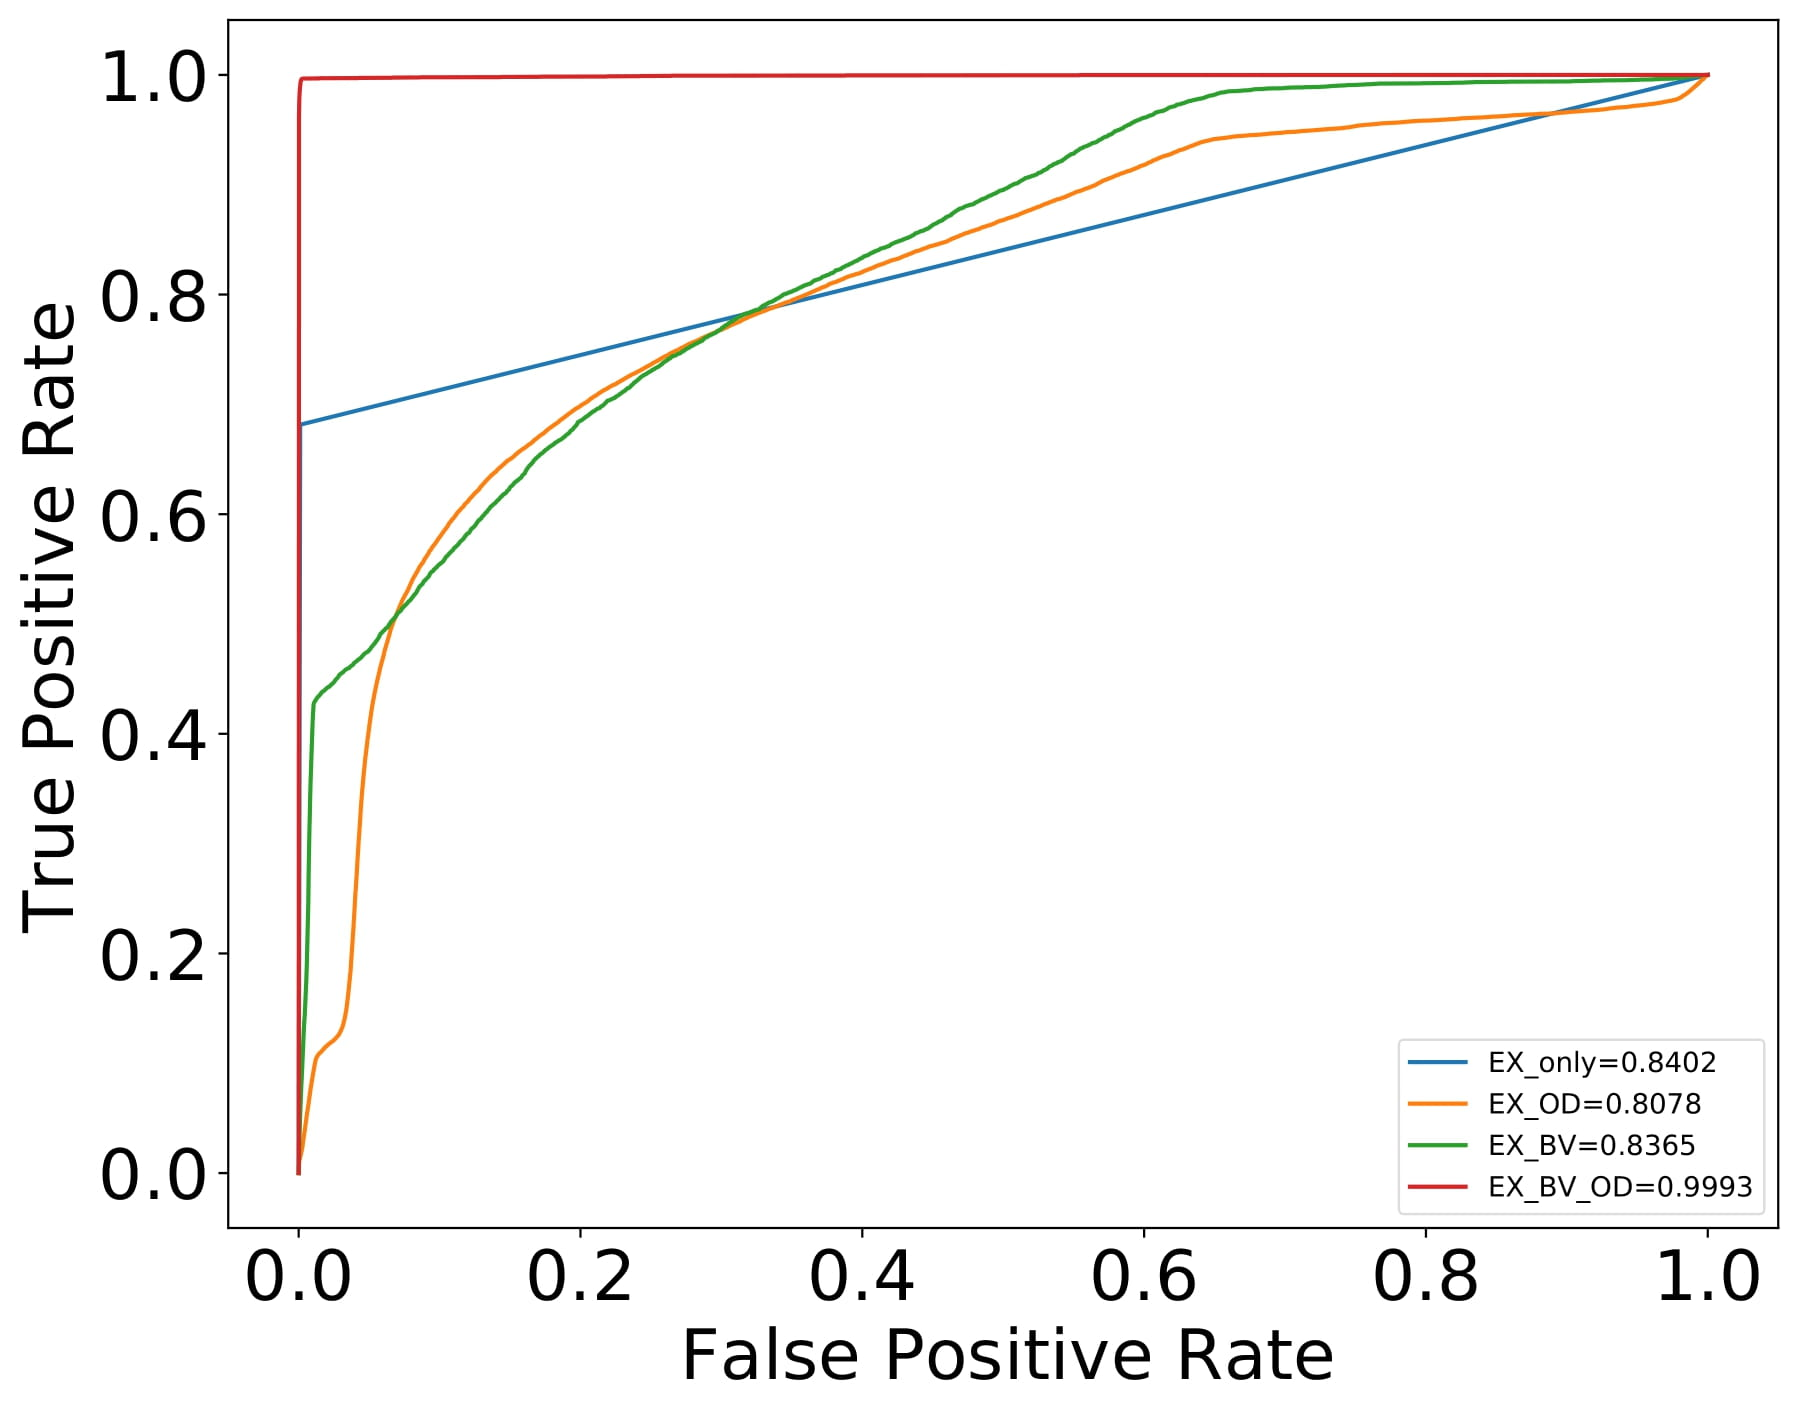
\includegraphics[width=14cm]{images/roc_auc_exudates.jpg}% This is a *.eps file
\end{center}
\caption{ROC-AUC curve for different experiments run on exudates segmentation. }
\label{fig:roc_auc_exudates}
\end{figure}

\begin{figure}
\begin{center}
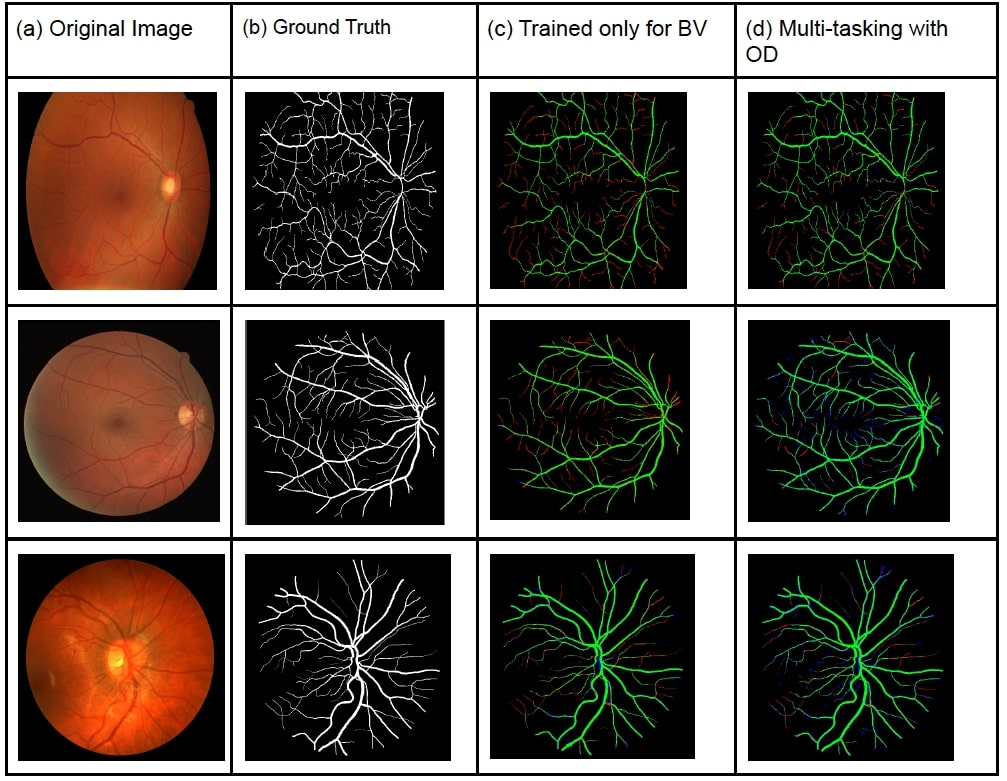
\includegraphics[width=14cm]{images/bv_results.jpg}% This is a *.eps file
\end{center}
\caption{A comparison of Blood Vessels segmentation results for HRF, DRIVE and CHASE\_DB (from top to bottom row) datasets with and without multi-tasking. The green pixels in the predicted image correspond to true positives, blue pixels correspond to false positives and  red pixels correspond to false negatives. An increase in F1-score score of 4.67\%,  3.31\%, 5.83\% is observed in HRF, DRIVE and CHASE\_DB respectively.}
\label{fig:bv_segmentation_results}
\end{figure}

Figure \ref{fig:bv_segmentation_results} shows  sample BV segmentation results with and without multi-tasking for HRF, DRIVE and CHASE\_DB. As evident from the figure, the increase in Dice score is due to less number of false negatives (red pixels) in the prediction (resulting in larger precision). Similarly Figures \ref{fig:od_segmentation_results}, \ref{fig:fovea_segmentation_results} and \ref{fig:exudates_segmentation_results} shows comparison of segmentation results for OD, Macula and exudates respectively.

\begin{figure}[h!]
\begin{center}
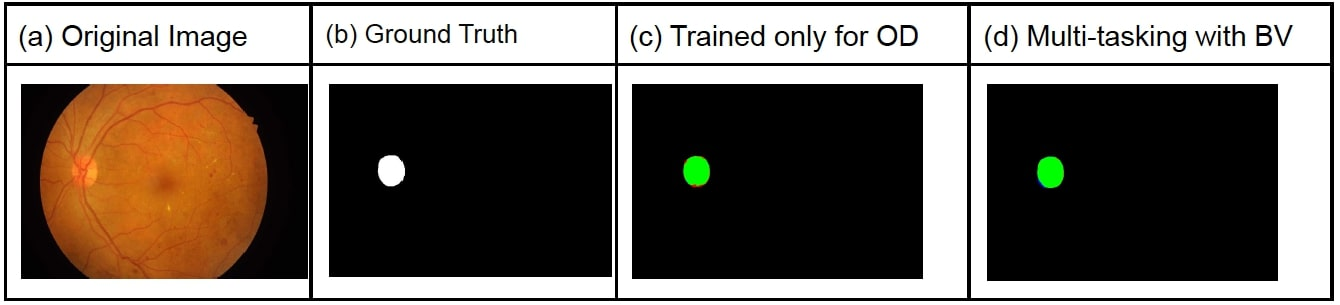
\includegraphics[width=15cm]{images/od_results.jpg}% This is a *.eps file
\end{center}
\caption{A comparison of OD segmentation results for the IDRiD dataset with and without multi-tasking. The green pixels in the predicted image correspond to true positives, blue pixels correspond to false positives and  red pixels correspond to false negatives. An increase in F1-score score of 9\% is observed.}

\label{fig:od_segmentation_results}
\end{figure}

\begin{figure}[h!]
\begin{center}
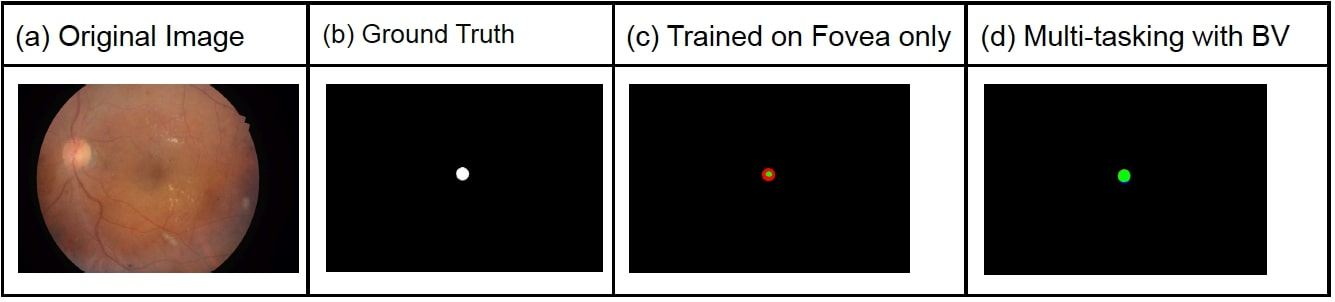
\includegraphics[width=15cm]{images/fovea_results.jpg}% This is a *.eps file
\end{center}
\caption{A comparison of Macula segmentation results for the IDRiD dataset with and without multi-tasking. The green pixels in the predicted image correspond to true positives, blue pixels correspond to false positives and  red pixels correspond to false negatives. An increase in F1-score score of 58\% is observed on this image.}
\label{fig:fovea_segmentation_results}
\end{figure}

\begin{figure}[h!]
\begin{center}
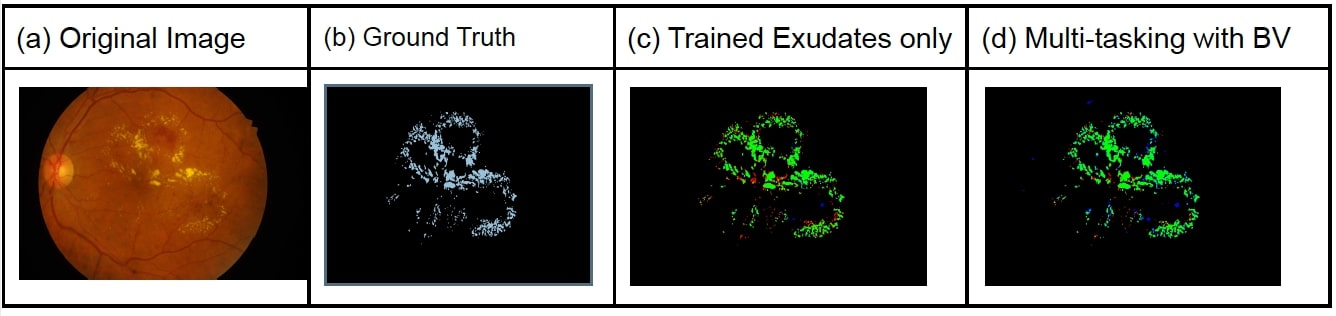
\includegraphics[width=15cm]{images/exudates_results.jpg}% This is a *.eps file
\end{center}
\caption{A comparison of exudates segmentation results for the IDRiD dataset with and without multi-tasking. The green pixels in the predicted image correspond to true positives, blue pixels correspond to false positives and  red pixels correspond to false negatives. An increase in F1-score score of 15\% is observed.}
\label{fig:exudates_segmentation_results}
\end{figure}

The improved performance with multi-tasking is a consequence of direct correlation between the two predicted structures. When trained together, the network is able to learn new hidden layer features that can contribute to the prediction of both structures.

When trained individually, the OD can easily be confused as exudates as both appear as white patches. In simultaneous segmentation, the network learns to discriminate Optic Disc and exudates, using some other features like shape for example, which improves the segmentation results for both.


Figure \ref{fig:zdim_vs_dice} shows the plot of validation Dice score Vs feature map dimension and Fig \ref{fig:channel_vs_dice}  shows Dice score as a function of  number of channels in the bottleneck layer. As evident from the graphs, we got the best results when the feature map dimension is $64\times64$ and the number of channels is 1024.

\begin{figure}[h!]
\begin{center}
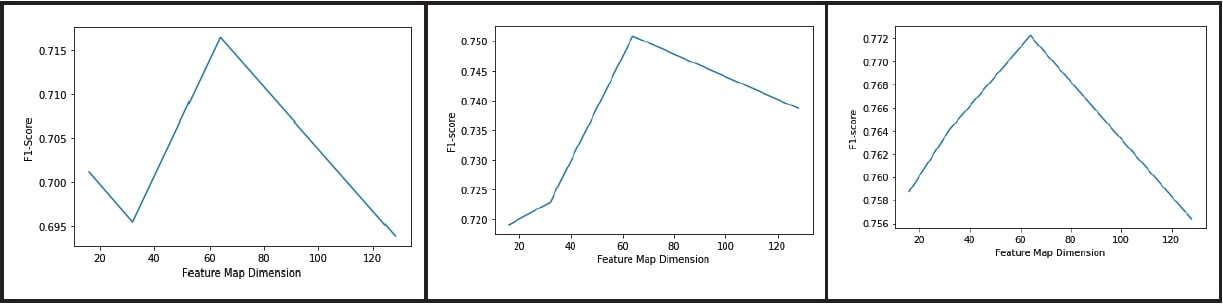
\includegraphics[width=15cm]{images/zdim_vs_dice.jpg}% This is a *.eps file
\end{center}
\caption{Plot of Dice score Vs Dimension of feature map in bottleneck layer for Blood vessel segmentation on DRIVE, CHASE\_DB and HRF (from left to right) datasets.}
\label{fig:zdim_vs_dice}
\end{figure}

\begin{figure}[h!]
\begin{center}
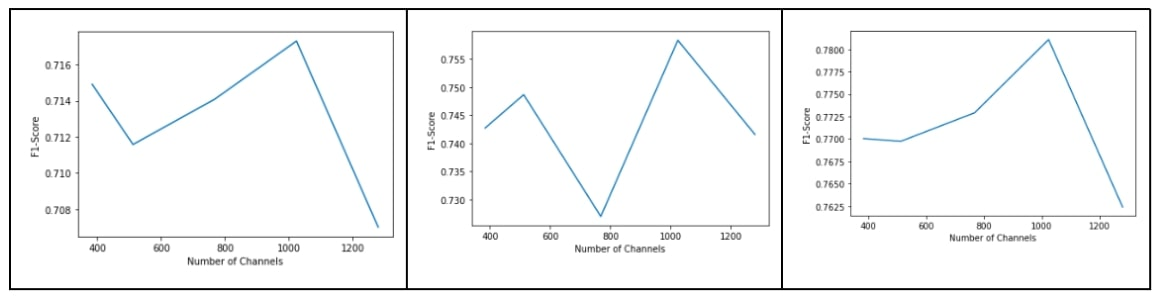
\includegraphics[width=15cm]{images/channel_vs_dice.jpg}% This is a *.eps file
\end{center}
\caption{Plot of Dice score Vs number of channels in bottleneck layer for Blood vessel segmentation on DRIVE, CHASE\_DB and HRF (from left to right) datasets.}
\label{fig:channel_vs_dice}
\end{figure}


Figure \ref{fig:bv_results_idrid} shows the results of BV segmentation on the IDRiD dataset using the model trained with images from  DRIVE, HRF and CHASE\_DB datasets. These segmentation results were used as BV ground truth of IDRiD images while training  for exudates in multi-tasking mode.

\begin{figure}[ht!]
\begin{center}
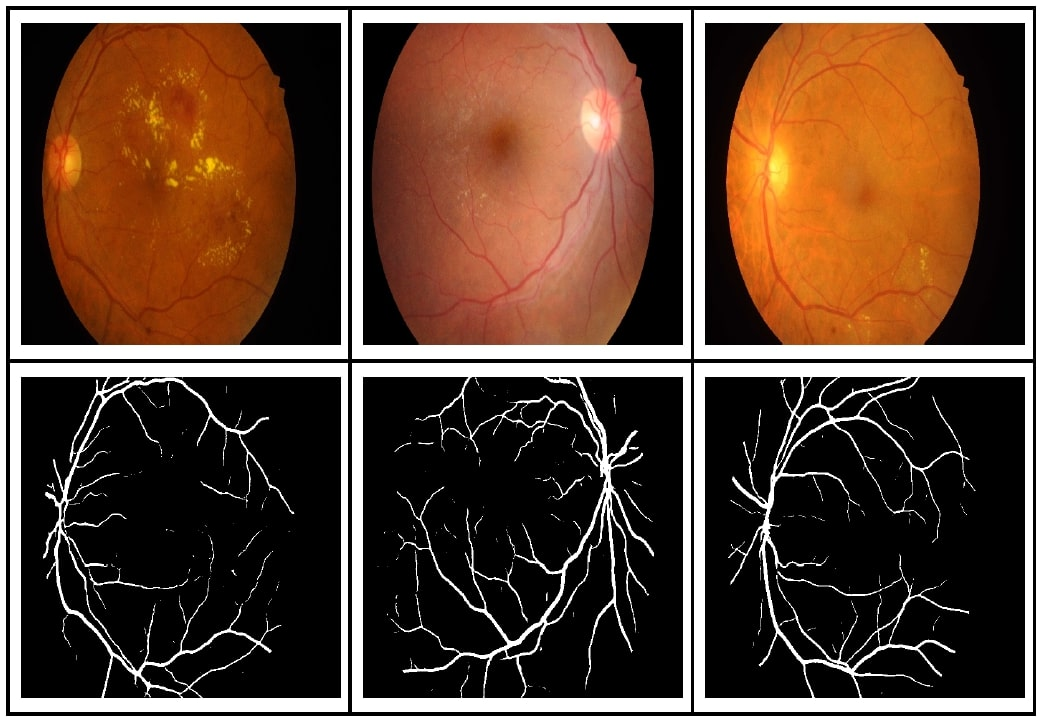
\includegraphics[width=15cm]{images/bv_results_idrid.jpg} % This is a *.eps file
\end{center}
\caption{BV segmentation results on the IDRiD dataset using the model trained with images selected from DRIVE, HRF and CHASE\_DB.}
\label{fig:bv_results_idrid}
\end{figure}


\begin{figure}[ht!]
\begin{center}
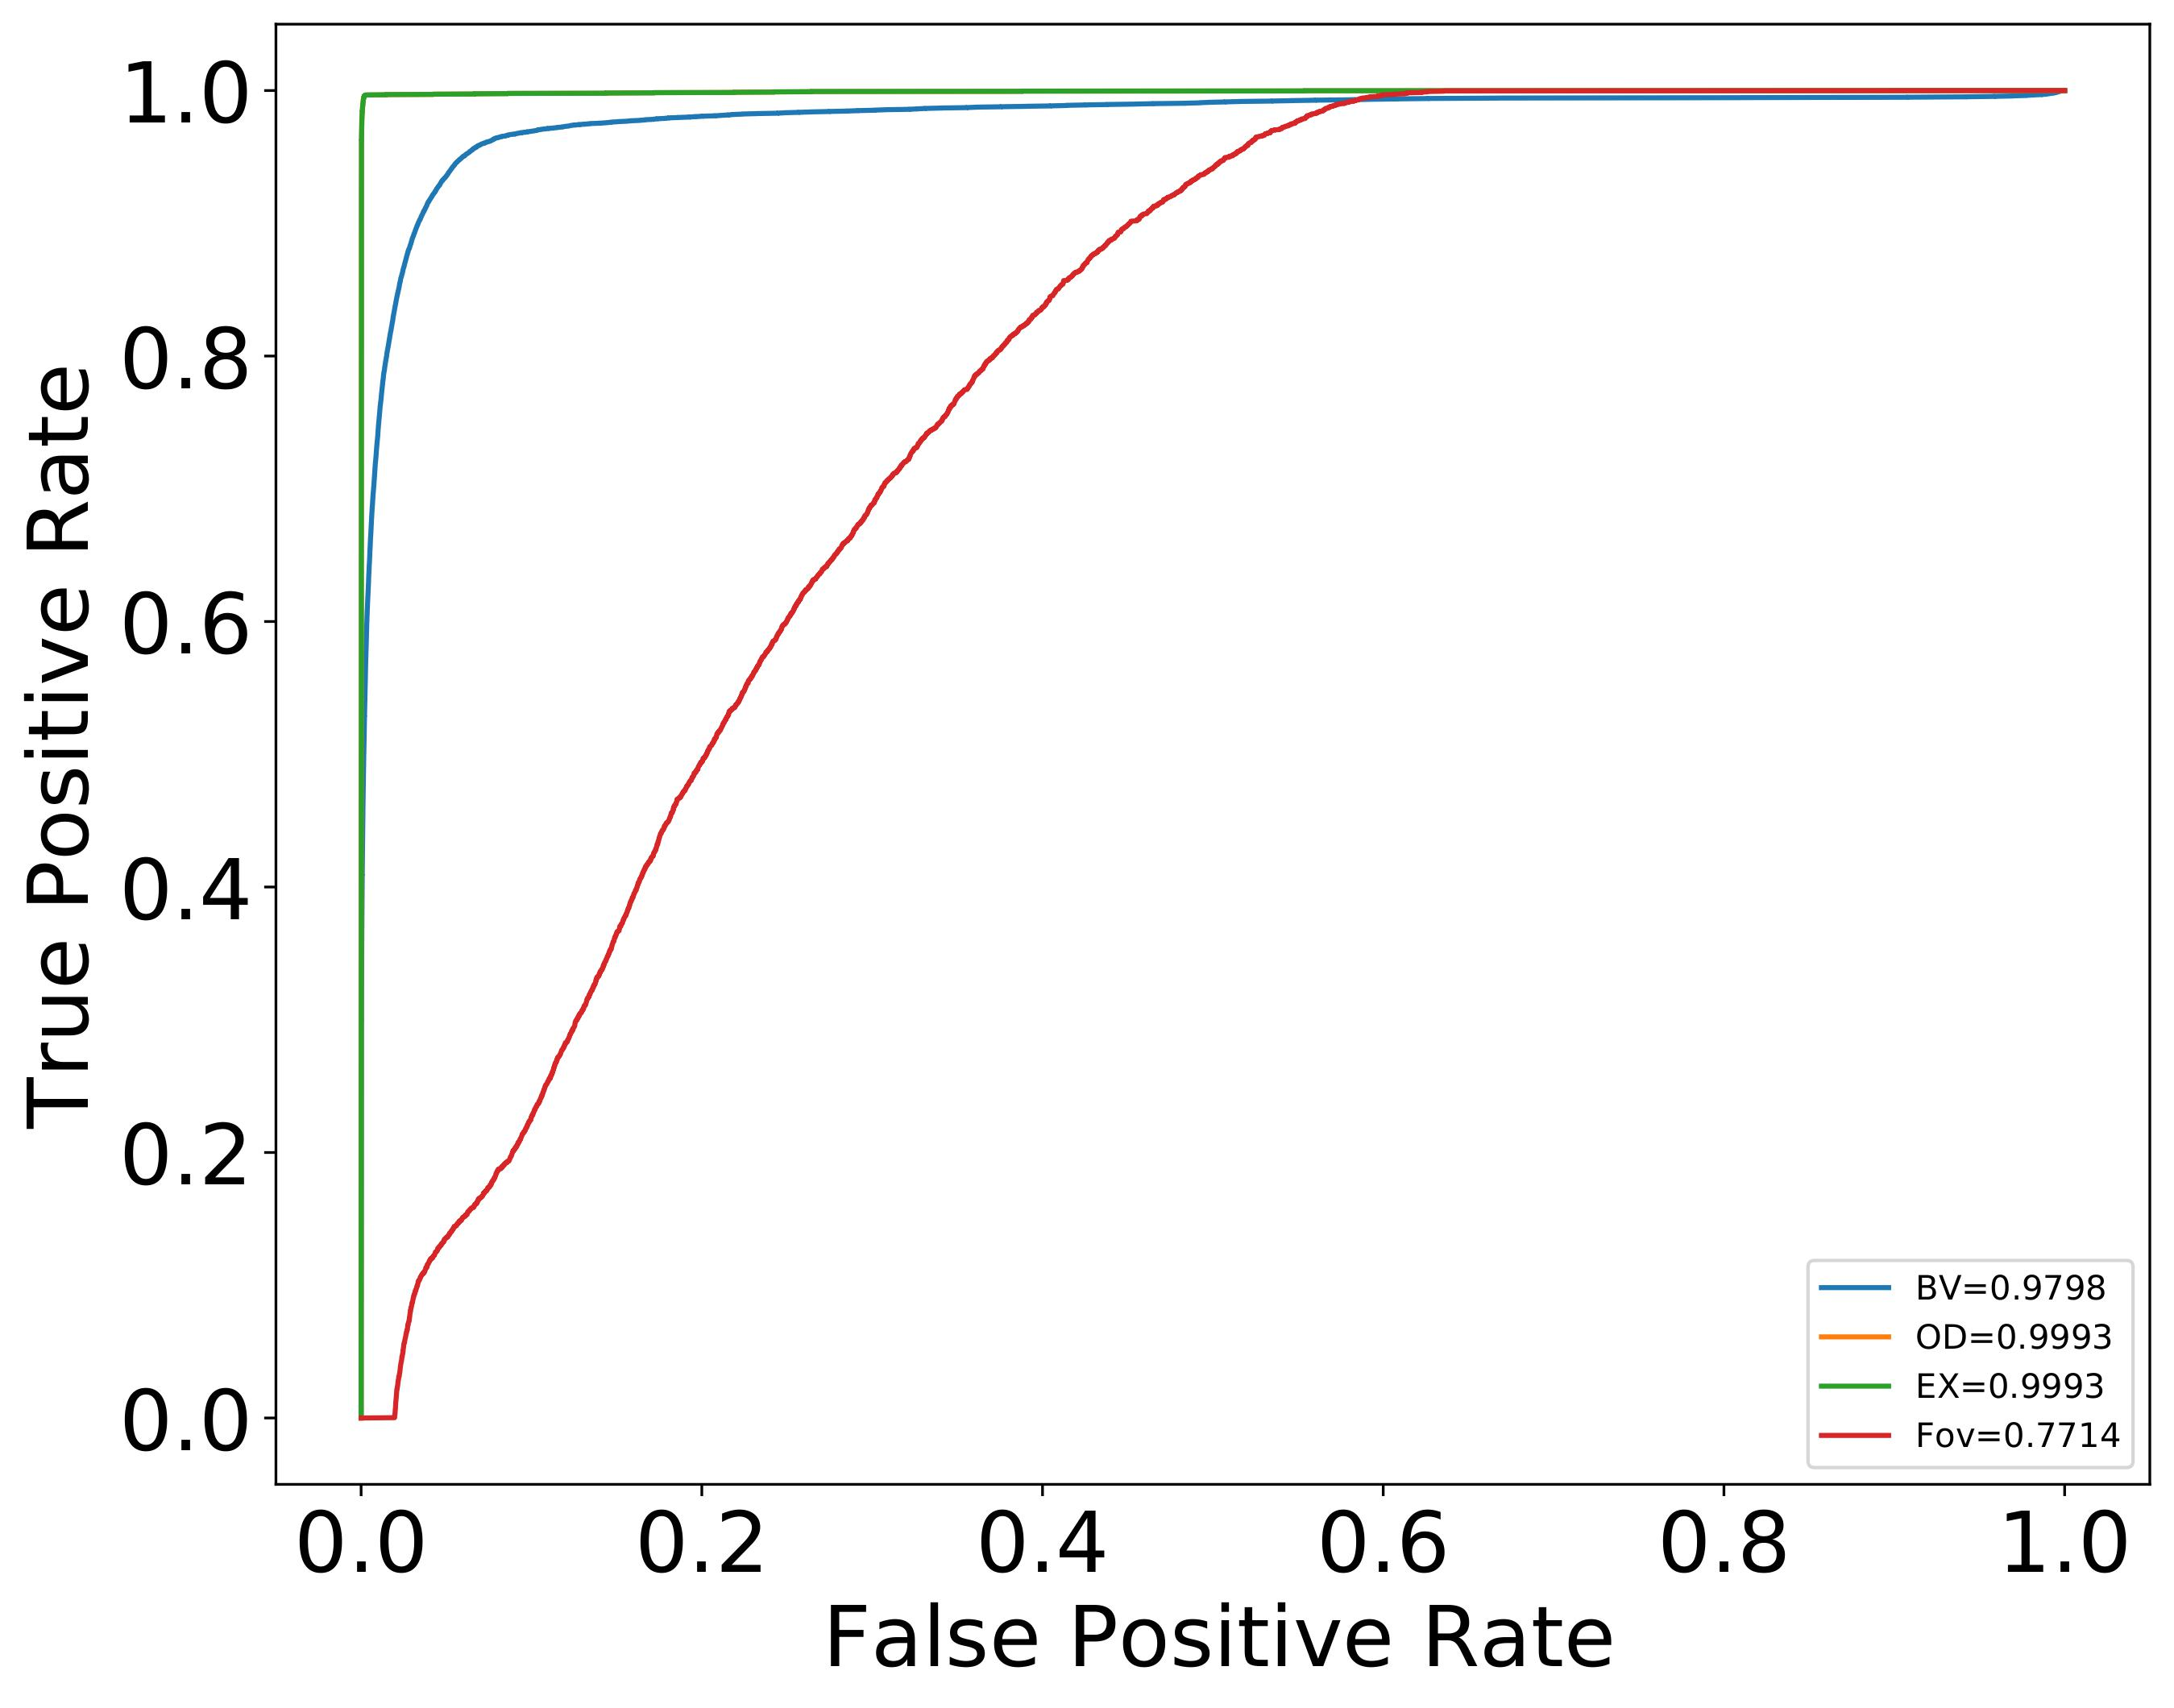
\includegraphics[width=15cm]{images/roc_all.jpg} % This is a *.eps file
\end{center}
\caption{ROC curve for all three structures BV, OD and Macula and the pathological indicator exudates. BV results are on the DRIVE test dataset. OD, Macula (FOV) and exudates (EX) are on the IDRiD dataset.
}
\label{fig:roc_auc}
\end{figure}

Figure \ref{fig:roc_auc} shows the Receiver Operating Characteristics(ROC) curve of the best results we got for all three structures BV, OD and Macula. Figure also shows the ROC curve for the pathological indicator exudates. BV segmentation results are on DRIVE test images. OD, Macula and exudates results are on the IDRiD dataset. As evident from the figure, the ROC curve for exudates, which is an indicator for early detection of many retinal diseases like DR, is encouraging. It is worth noting that we got these improved results as a consequence of multi-tasking with BV and OD.


Table \ref{tab:result_comparison_ex} shows comparison of our exudates segmentation results with state-of-the-art techniques. AUC of our segmentation result is better than state-of-the-art DL methods \cite{kou2020enhanced} and more significantly our prediction time is significantly better than the state-of-the-art DL approaches. This is because, we are doing whole image segmentation in single forward-pass, where as many DL state-of-the-art approaches approaches used patch-wise training and hence prediction of a single image takes longer as the network needs to predict on each patch and finally all the predictions needs to be combined together to get the overall all segmentation results for the image.  We believe that the AUC can further be improved by adding more data-augmentation techniques and also by including more images in the original training set. Our improvement in AUC is attributed to faster learning of more generalized features as a consequence of multi-tasking. Another major advantage of our approach is that we get segmentation of two additional different structures, BV and OD, along with exudates segmentation. \cite{nur2018exudate} got an accuracy of 99.33\% by removing the OD first and then obtaining the salient regions using intensity thresholding. The challenge with this method is that the threshold can vary from dataset to dataset and further the accuracy also depends on the OD removal step.

\begin{table}[!h]
\centering
\caption{Comparison of exudates segmentation results of our approach with other state-of-the-art approaches on IDRiD dataset. As we are predicting on whole images, our prediction time is much faster (about 12 times) compared to other state-of-the-art techniques on the IDRiD dataset. FCN:Fully Convolutional Networks, ACC:Accuracy, SUP:Supervised, UNSUP: Unsupervised}
\label{tab:result_comparison_ex}
\vspace{2mm}
\begin{tabular}{|p{2.5cm}|p{3.3cm}|p{1.4cm}|p{2.4cm}|p{1.2cm}|p{1.5cm}|p{2cm}|}
\hline
\textbf{Author/ Year} &  \multicolumn{3}{|c|}{\textbf{Approach}}   & \multicolumn{3}{|c|}{\textbf{Performance Metrics}}  \\
\cline{2-7}
&\textbf{Method} &\textbf{SUP/ \newline UNSUP} &   \textbf{Patch-wise/ \newline Whole Image} &\textbf{AUC} & \textbf{ACC(\%)} & \textbf{Prediction} \newline \textbf{time(sec)}\\
\hline
%
\cite{kaur2022uniconv}  & UNet with \newline InceptionV3 & SUP & &  - & 99.83 & - \\
\hline
\cite{hamad2020exudates}  & FCM Clustering & UNSUP & Patch-wise \newline $(256 \times 256)$  & -  & 99.2 & 30 \\
\hline

\cite{kou2020enhanced}  & ER-UNet &SUP& Patch-wise &   0.9801 & 98.00 & 37.3 \\
\hline
\cite{guo2020bin}  &  Deeplab-V2 \newline with Bin loss &SUP& Patch-wise \newline ($51\times51$) & 0.9162 & 99 & - \\
\hline
\cite{nur2018exudate}  & Saliency based & UNSUP& Patch-wise \newline ($32\times32$) & - & 99.33 & - \\
\hline
Our approach & Modified U-NET \newline Multi-tasking & SUP & Whole Image & \textbf{0.9993} & \textbf{99.42} & \textbf{2-3} \\

\hline
\end{tabular}
\end{table}

Figure \ref{fig:exudates_comparison} shows comparison of exudates segmentation results of the proposed approach with the approach mentioned in \cite{guo2020bin} for some sample images. Even though we got better  accuracy (99.42) and AUC (0.9993) when averaged over the entire test images, our model failed to capture very small exudates, as shown in the second row of Figure \ref{fig:exudates_comparison}. This is because such finer exudates get removed when the image is resized from original size of $4288 \times 2848$ to $768 \times 512$.

\begin{figure}[ht!]
\begin{center}
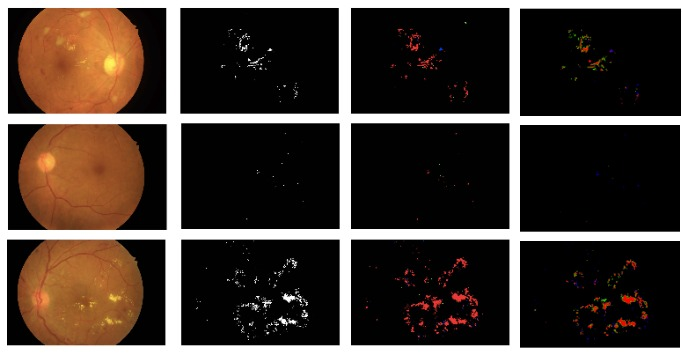
\includegraphics[width=15cm]{images/exudates_comparison.jpg} % This is a *.eps file
\end{center}
\caption{Comparison of exudates segmentation result of the proposed approach with \cite{guo2020bin}. Each column from left shows the original image, ground truth segmentation results of \cite{guo2020bin} and segmentation result of proposed approach. Color code used is kept the same as in \cite{guo2020bin} for ease of comparison. Red: True Positive, Green: False Positive, Blue: False Negative.}
\label{fig:exudates_comparison}
\end{figure}


Table \ref{tab:result_comparison_bv} shows the comparison of our BV segmentation results with the state-of-the-art techniques. As evident from the table accuracy (95.89\%) of our approach on the DRIVE dataset is better than the currently reported state-of-the-art and AUC is close to the state-of-the-art. Dice scores on all three dataset are lower than patch based state-of-the-art techniques. However, since we train on whole images, both training and prediction time is about 20 times faster than patch based deep learning approaches.

\begin{table}[!h]
\centering
\caption{Comparison of BV segmentation results of our approach with other state-of-the-art approaches.ACC: Accuracy }
\label{tab:result_comparison_bv}
\vspace{2mm}
\begin{tabular}{|p{3.5cm}|p{3cm}|p{2.5cm}|p{2cm}|p{1cm}|p{0.9cm}|p{1cm}|}
\hline
\textbf{Author/ Year} &  \textbf{Approach} & Patch-wise/ \newline Whole Image & \textbf{Dataset} & \multicolumn{3}{|c|}{\textbf{Performance Metrics}}  \\
\cline{5-7}
&&&& \textbf{Dice} & \textbf{AUC} & \textbf{ACC}\\
\hline
\cite{xu2021retinal} & Residual Attention \newline with ASPP and \newline Deep Supervision & Patch-wise \newline ($64 \times 64$)  & DRIVE & - & 0.97 &95.9 \\
\hline

\cite{liu2021construction} & Hand-crafted features \newline with MLP & Whole Image & DRIVE & - & - & 95.82 \\
\hline

\cite{jiang2018retinal} & FCNN \newline Transfer learning & Patch-wise \newline ($50\times50$) & DRIVE \newline HRF \newline CHASE\_DB & - & 0.98 \newline 0.97 \newline 0.98 &- \\
\hline
\cite{joshua2020blood} & U-Net &  Whole Image & DRIVE \newline HRF \newline CHASE\_DB & 87.62 \newline  85.11 \newline 85.69 & -  & -\\
\hline

\cite{park2020m} &  M-GAN  & Path-wise ($48 \times 48$) & DRIVE \newline HRF \newline CHASE\_DB & 83.24 \newline 79.92 \newline 81.10 & - & -\\
\hline

\cite{sun2021robust} &  Data \newline Augmentation & Whole Image & DRIVE  \newline CHASE\_DB & 82.09 \newline 75.65 & - & -\\
\hline
\cite{adapa2020supervised} &  Zernike Moment & Whole Image & DRIVE  & - & - & 94.5 \\
\hline
\cite{dash2020retinal} & \underline{\textbf{Preprocessing}}: \newline CLACHE \newline Gabor \newline Hessian \newline  \underline{\textbf{Segmentation}}:\newline k-means \newline \underline{\textbf{Post Processing}}:\newline Morphological cleaning & Whole Image & DRIVE \newline CHASE\_DB  & - & - & 95.2 \newline 95 \\
\hline
Our approach & Multi-tasking \newline using U-NET & Whole Image & DRIVE \newline HRF \newline CHASE\_DB  & 80.31 \newline 81.66\newline 80.45 & 0.98 & 95.89 \\
\hline
\end{tabular}
\end{table}

\section{Conclusion}
In this work, we illustrate the efficacy of  modified multi-tasking U-Net for segmenting Blood Vessels, Optic Disc, Macula and exudates in fundal images.  The proposed approach resulted in  a peak increase of 15\% in Dice score for exudates segmentation compared to the individual segmentation result with the same architecture. Using the proposed approach, we are able to get a state-of-the-art accuracy of 95.89\% on DRIVE test images which is 0.7\% greater than one of the recently reported results. With our proposed method, the prediction times on the images are significantly lesser (12 times)  compared to most other deep learning methods. In addition to this increased speed in prediction, we could improve the AUC and Accuracy for exudates from 0.9801 to 0.9993 and 99.33\% to 99.42\% on the IDRiD test dataset.

\section*{Conflict of Interest Statement}
%All financial, commercial or other relationships that might be perceived by the academic community as representing a potential conflict of interest must be disclosed. If no such relationship exists, authors will be asked to confirm the following statement:
The authors declare that the research was conducted in the absence of any commercial or financial relationships that could be construed as a potential conflict of interest.

\section*{Author Contributions}

Sunil Kumar Vengalil and Bharath K contributed in conceptualization, investigation and to develop the methodology. Bharath K carried out the implementation and ran all the experiments mentioned in this work. Both Bharath K and Sunil Kumar Vengalil contributed equally in writing and formatting the manuscript. Neelam Sinha supervised the work and was involved in writing-reviewing-editing. Neelam Sinha validated the work and provided the resources.

\section*{Funding}
This work was funded by Machine Intelligence and Robotics Center (MINRO) Project GoK, IIITB. It is supported by Karnataka Innovation \& Technology Society, Dept. of IT, BT and S\&T, Govt. of Karnataka vide GO No. ITD 76 ADM 2017, Bengaluru; Dated 28.02.2018

%\section*{Acknowledgments}
%This is a short text to acknowledge the contributions of specific colleagues, institutions, or agencies that aided the efforts of the authors.
%
%\section*{Supplemental Data}
% \href{http://home.frontiersin.org/about/author-guidelines#SupplementaryMaterial}{Supplementary Material} should be uploaded separately on submission, if there are Supplementary Figures, please include the caption in the same file as the figure. LaTeX Supplementary Material templates can be found in the Frontiers LaTeX folder.

\section*{Data Availability Statement}
\begin{enumerate}
\item Digital Retinal Images for Vessel Extraction Dataset (DRIVE) dataset is available at \newline \url{http://www.isi.uu.nl/Research/Databases/DRIVE/}
\item High-Resolution Fundus (HRF) Image Database \newline \url{https://www5.cs.fau.de/research/data/fundus-images/}
\item CHASE\_DB1 Retinal Image Database \url{https://www.idiap.ch/software/bob/docs/bob/bob.db.chasedb1/master/index.html}
\item Indian Diabetic Retinopathy Image Dataset (IDRiD) \url{https://idrid.grand-challenge.org/}
\end{enumerate}

\bibliographystyle{Frontiers-Harvard} %  Many Frontiers journals use the Harvard referencing system (Author-date), to find the style and resources for the journal you are submitting to: https://zendesk.frontiersin.org/hc/en-us/articles/360017860337-Frontiers-Reference-Styles-by-Journal. For Humanities and Social Sciences articles please include page numbers in the in-text citations
%\bibliographystyle{Frontiers-Vancouver} % Many Frontiers journals use the numbered referencing system, to find the style and resources for the journal you are submitting to: https://zendesk.frontiersin.org/hc/en-us/articles/360017860337-Frontiers-Reference-Styles-by-Journal
\bibliography{test}

%%% Make sure to upload the bib file along with the tex file and PDF
%%% Please see the test.bib file for some examples of references

% \section*{Figure captions}

%%% Please be aware that for original research articles we only permit a combined number of 15 figures and tables, one figure with multiple subfigures will count as only one figure.
%%% Use this if adding the figures directly in the mansucript, if so, please remember to also upload the files when submitting your article
%%% There is no need for adding the file termination, as long as you indicate where the file is saved. In the examples below the files (logo1.eps and logos.eps) are in the Frontiers LaTeX folder
%%% If using *.tif files convert them to .jpg or .png
%%%  NB logo1.eps is required in the path in order to correctly compile front page header %%%


%%% If you are submitting a figure with subfigures please combine these into one image file with part labels integrated.
%%% If you don't add the figures in the LaTeX files, please upload them when submitting the article.
%%% Frontiers will add the figures at the end of the provisional pdf automatically
%%% The use of LaTeX coding to draw Diagrams/Figures/Structures should be avoided. They should be external callouts including graphics.

\end{document}




